\section{Harp PageRank}

\FILENAME\

For this exercise you will implement PageRank on Harp framework.

\subsection{Deliverables}
Zip your source code and output as username\_harp-pagerank.zip. Please submit
this file to the Canvas Assignments page.

\subsection{Evaluation}
The point total for this exercise is 6, where the distribution is as follows:


\begin{itemize}
\item Completeness of your code (5 points)
\item Correct output (1 point)
\end{itemize}

\subsection{Prerequisites}
From now on, you don't need the old VM. To avoid any conflict and
inconvenience, we have prepared a new VM (ubuntu 16.04) for you. The link will
be posted on canvas. All necessary tools/libaries such Maven, JDK, Github,
Hadoop 2.6.0, Harp are configured and ready for use. Intellij is installed as
well. You can also use your own VM. But you will need to setup those
tools/libraries by yourself. Some tutorials are available at the harp
website. Here this instruction is based on the configurations in
this new VM.

\begin{figure}[!htbp]
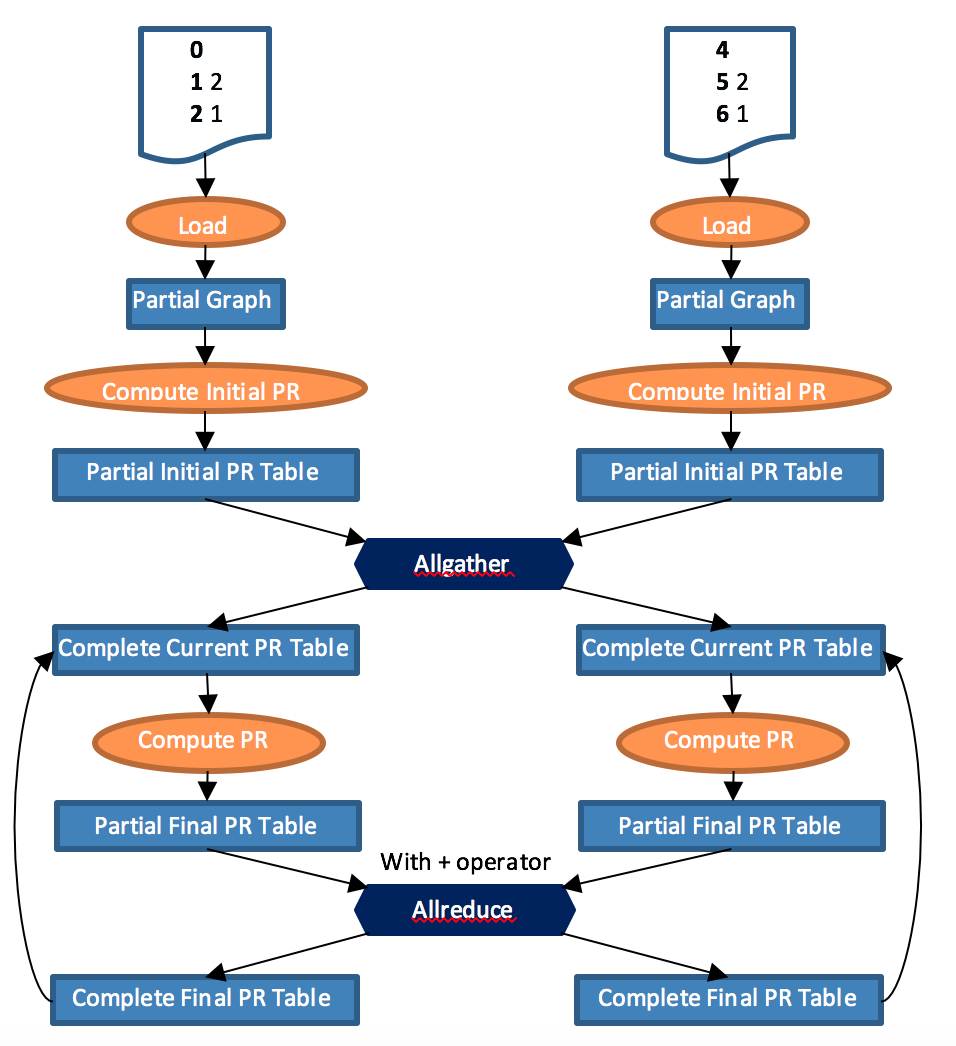
\includegraphics[width=6cm,height=8cm]{section/icloud/assignment/exercise7/p8}
\centering
\caption{Harp PageRank Architecture}
\end{figure}

\subsection{HarpPageRank Implementation}
Most of the code is completed for you and your task will be to perform the
\textbf{Compute PR} step in the above diagram. The code for this can be found
in \textbf{simplepagerank/PageRankMapper.java}

\lstinputlisting[language=Java]{section/icloud/assignment/exercise7/computePartialPR.java}

\subsection{Compilation and Running}
\begin{itemize}
\item To make the modification to the code, you can use Intellij IDE or linux
  terminal. The source code is located at 
\begin{lstlisting}[language=bash]
/home/cc/Documents/harp/harp-tutorial-app/src/main/java/edu/iu/simplepagerank
\end{lstlisting}
\item To compile the code, type the following commands in terminal
\begin{lstlisting}[language=bash]
$ cd $HARP_ROOT_DIR
$ mvn clean package
\end{lstlisting}

\item If hadoop is not started, start hadoop by:
\begin{lstlisting}[language=bash]
$ $HADOOP_HOME/sbin/start-dfs.sh
$ $HADOOP_HOME/sbin/start-yarn.sh
\end{lstlisting}

Then you can view the web UI at  localhost:50070 and localhost:8088

\item We prepared the input dataset (input5K-2partitions) for you. Use the
  following command to put it to hdfs. Please note there is a "dot" at the end
    of the second command.

\begin{lstlisting}[language=bash]
$ cd $HARP_ROOT_DIR/data/tutorial/simplepagerank
$ hdfs dfs -put input5K-2partitions .
\end{lstlisting}
\item Run the program:
\begin{lstlisting}[language=bash]
$ cd $HARP_ROOT_DIR
$ hadoop jar harp-tutorial-app/target/harp-tutorial-app-1.0-SNAPSHOT.jar edu.iu.simplepagerank.HarpPageRank input5K-2partitions output5k 5000 10
\end{lstlisting}

This will run PageRank against input2K-2partitions dataset. It has 5000 URLs in total. The program will run 2 parallel map tasks for 10 iterations.  If you want to launch N map tasks, you need to divide the dataset into N partitions.

\item To get the output, perform the following commands to get the output to the Desktop. Then you can submit it to canvas.
\begin{lstlisting}[language=bash]
$ hdfs dfs -get output5k /home/cc/Desktop
\end{lstlisting}
\end{itemize}
